%%%%%%%%%%%%%%%%%%%%%%%%%%%%%%%%%%%%%%%%%%%%%%%%%%%%%%%%%%%%%%%%%%%%%%
% Problem statement
\begin{statement}[
  problempoints=70,
  timelimit=1 second,
  memorylimit=512 MiB,
]{Birmingham}

\setlength\intextsep{-0.1cm}
\begin{wrapfigure}[6]{r}{0.27\textwidth}
\centering
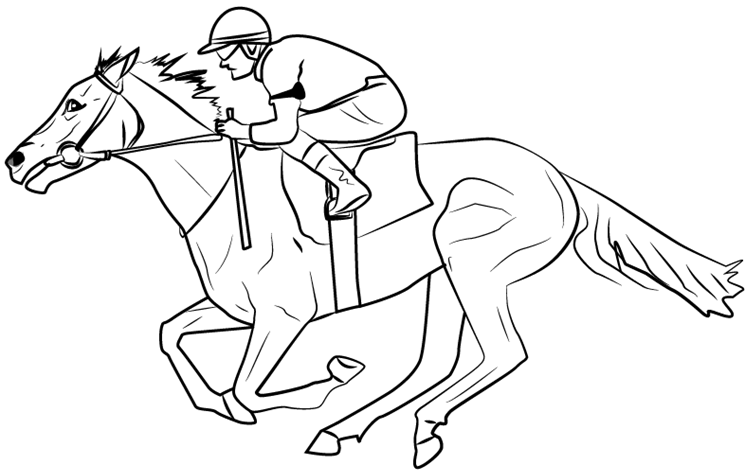
\includegraphics[width=0.27\textwidth]{img/birmingham.png}
\end{wrapfigure}

It is well known that all horse races in Birmingham are fixed days in advance.
It is a little less known that certain people that fix these races (and
thereby know the winner) start spreading that information around the city the
next day.

The first day after the meeting, all people that know the information about the
winner start sharing that information with all people that live at most $K$
steps away from their house.

The second day after the meeting, all people that know the information about
the winner start sharing that information with all people that live at most
$2 \cdot K$ steps away from their house.

In general, $X$-th day after the meeting, all people that know the information
about the winner start sharing that information with all people that live at
most $X \cdot K$ steps away from their house.

We can represent Birmingham as a graph where vertices represent the houses and
edges represent bidirectional roads which connect these houses. Houses are
indexed with increasing integers from $1$ to $N$ and we say that a person
can travel each road in a single step. It is possible to reach each house
from each other house by traversing a sequence of roads.

Your task is to determine, for each house, on which day will the information
about the race winner reach it.

%%%%%%%%%%%%%%%%%%%%%%%%%%%%%%%%%%%%%%%%%%%%%%%%%%%%%%%%%%%%%%%%%%%%%%
% Input
\subsection*{Input}
The first line contains four integers $N$, $M$, $Q$ and $K$ $(1 \le N, Q, K \le
100\ 000, Q \le N, 1 \le M \le 200\ 000)$, the number of houses in
Birmingham, the number of roads in Birmingham, the number of people that were
present on the secret meeting and the number $K$ from task description.

The next line contains $Q$ integers where the $i$-th integer represents
the index of a house where the $i$-th person from the secret meeting lives in.

The $i$-th of the next $M$ lines contains integers $A_i$ and $B_i$ $(1
\le A_i, B_i \le N, A_i \neq B_i)$, which denote that the $i$-th road
connects houses with indices $A_i$ and $B_i$.

%%%%%%%%%%%%%%%%%%%%%%%%%%%%%%%%%%%%%%%%%%%%%%%%%%%%%%%%%%%%%%%%%%%%%%
% Output
\subsection*{Output}
Output $N$ numbers where the $i$-th number represents on which day after the
meeting will the person living in house with index $i$ find out who will win
the race.  If the person living in that house was present on the secret
meeting, output $0$ instead.

%%%%%%%%%%%%%%%%%%%%%%%%%%%%%%%%%%%%%%%%%%%%%%%%%%%%%%%%%%%%%%%%%%%%%%
% Scoring
\subsection*{Scoring}
In the test cases worth a total of $20$ points, it will hold $K=1$, $1 \le N, Q
\le 100$ and $1 \le M \le 200$.\\
In the test cases worth an additional $15$ points, it will hold $1 \le N, Q \le
100$ and $1 \le M \le 200$.

%%%%%%%%%%%%%%%%%%%%%%%%%%%%%%%%%%%%%%%%%%%%%%%%%%%%%%%%%%%%%%%%%%%%%%
% Examples
\subsection*{Examples}
\begin{tabularx}{\textwidth}{X'X'X}
\sampleinputs{test/birmingham.dummy.in.1}{test/birmingham.dummy.out.1} &
\sampleinputs{test/birmingham.dummy.in.2}{test/birmingham.dummy.out.2} &
\sampleinputs{test/birmingham.dummy.in.3}{test/birmingham.dummy.out.3}
\end{tabularx}

\textbf{Clarification of the third example:}
The figure represents a graph from the third example. Since houses $1$, $2$, $3$
and $5$ are at most two steps away from house $6$, people living in them will
find out about the winner the day after the meeting. Person living in house $4$
will find out about the winner two days after the meeting.

\setlength\intextsep{-0.5cm}
\begin{wrapfigure}{c}{\textwidth}
\centering
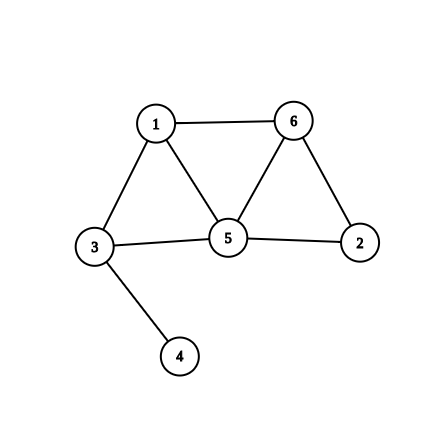
\includegraphics[width=0.4\textwidth]{graph.png}
\end{wrapfigure}

%%%%%%%%%%%%%%%%%%%%%%%%%%%%%%%%%%%%%%%%%%%%%%%%%%%%%%%%%%%%%%%%%%%%%%
% We're done
\end{statement}

%%% Local Variables:
%%% mode: latex
%%% mode: flyspell
%%% ispell-local-dictionary: "croatian"
%%% TeX-master: "../hio.tex"
%%% End:
